Many real-world applications ranging from search engines to conversational agents rely on the ability to uncover new relationships from existing knowledge.
Relation extraction (RE) and knowledge graph link prediction (KGLP) are two learning tasks that are both very popular and that center around inferring new information from existing facts.
RE is a textual inference task that aims to discover the relationship between two entities (termed the subject and the object, respectively) in a sentence.
For instance, given the sentence ``\texttt{Miami is in Florida}'' with subject \texttt{Miami} and object \texttt{Florida}, RE methods have to predict the relationship \texttt{locatedIn}.
RE is important because it is used for downstream applications (e.g., knowledge graph [KG] population) and the underlying ideas are also applicable to other related important problems such as question answering. Knowledge graph link prediction (KGLP), on the other hand, aims to populate KGs by uncovering the set of correct answers (i.e., objects) to questions comprised of graph nodes (i.e., subjects) and edges (i.e., relations) in the form of \texttt{(subject,relation,?)} triples.
The uncovered answers are used to populate the KG by establishing connections between subjects and objects using relations.
For instance, the answers \texttt{Florida} and \texttt{USA} to the question \texttt{(Miami,LocatedIn,?)}, form two new connections in the KG: \texttt{(Miami,LocatedIn,Florida)} and \texttt{(Miami,LocatedIn,USA)}, respectively.

Relation extraction and knowledge graph link prediction are inherently related.
To illustrate, let $s$, $o$ and $r$ represent the subject, object, and relation, respectively, that are contained in a sentence.
RE methods infer the relation $r$ given the sentence, the subject $s$, and the object $o$.
Comparatively, KGLP methods utilize $r$ and $s$ to predict a set of objects $O$ that is expected to include $o$. In our previous examples, $O$ \texttt{= \{Florida, USA\}} and $o$ \texttt{= Florida}, respectively.

Several methods have been proposed to boost the performance of RE models by jointly training over both RE and KGLP tasks.
% Both RE and KGLP have garnered substantial interest and popularity in recent years, and several methods have been proposed to boost the performance of RE methods with the additional supervision of a KGLP model.
% proposed to utilize the additional supervision provided by a KGLP method to boost the performance of a RE model.
% Both RE and KGLP have garnered substantial interest and popularity in recent years, and many method have been proposed to leverage their similarities to improve performance by jointly training over both tasks.
% Both RE and KGLP have garnered substantial interest and popularity in recent years, and several methods have been proposed to leverage their similarities to improve performance by jointly training over both tasks.
However, these approaches typically require KGLP pre-training \citep[e.g.]{weston-2013, lfds}, exhibit constrained parameter sharing \citep[e.g.]{weston-2013, lfds}, or predominately attend over both problems through custom attention mechanisms \citep[e.g.,][]{bag_re_kglp,han,long_tail}.
% While both RE and KGLP have garnered substantial interest and popularity in recent years, less work leverages the aforementioned relationship between the two. 
% We propose a method that leverages this relationship and manages to improve RE performance, by using knowledge acquired while learning to do well on the KGLP task.
% To illustrate the similarities between RE and KGLP, 
% Leveraging additional supervision encapsulated in KGs to improve the performance of RE models has previously been explored by using KGLP methods to {\em fact-check} (i.e., to determine the correctness of the resulting subject-relation-object triple).
% While both RE and KGLP have garnered substantial interest and popularity in recent years, less work leverages
% work has been proposed that attempts to leverage 
% the aforementioned relationship between the two. 
% We propose a method that does exactly that, and also manages to outperform existing methods. but before we summarize our contribution, let us explain what we mean when we say that the two tasks are similar.
% RE predictions \citep[e.g.,][]{weston-2013}.
% While such methods have achieved strong performance, they typically require KGLP pre-training and only allow for very limited information sharing between the two tasks.
% This is because the RE model cannot use any information provided by the KGLP model while producing a ranked list of predictions.
% The KGLP model effectively only acts as a {\em reranker} for the ranked list that the RE model generates.
% Moreover and perhaps most importantly, these methods are not generalizable to arbitrary KGLP models as they are often designed around a specific class of KGLP approaches, 
% nor do they necessarily
% I want to say:
% - previous approaches 
% While such methods have achieved strong performance, they typically require KGLP pre-training, and predominately explicitly attend over both tasks through complicated dual attention mechanisms \citep[e.g.,][]{bag_re_kglp,han,long_tail}.
% and are incapable of reasoning over more expressive recent link prediction approaches.
% Although some prior methods also reason over RE and KGLP problems without using such attention mechanisms, they have to trade-off of very limited information sharing between the two tasks (e.g. \cite{weston-2013}), or learning a single task at a time (e.g. \cite{weston-2013, lfds}).
Although some prior methods also reason over RE using KGLP without such attention mechanisms, they either severely restrict information sharing between the two tasks \citep[e.g.,][]{weston-2013}, or only learn a single task at a time \citep[e.g.,][]{lfds,weston-2013} rather than learning both tasks jointly.
Moreover, these frameworks only support a limited class of KGLP models that can be reframed as inferring relations from subject and objects.
This constraint excludes recent KGLP methods which perform significantly better, but cannot be reformulated to satisfy the restriction.
An ideal framework should support arbitrary RE and KGLP methods, including the significantly more expressive and stronger performing recent KGLP approaches.
Additionally, such a framework should enable RE models to benefit from KGLP models with minimal changes to the underlying RE and KGLP methods.

\begin{figure*}[t]
    \centering
    % \includegraphics[width=1.0\textwidth]{images/coper_horizontal.pdf}
    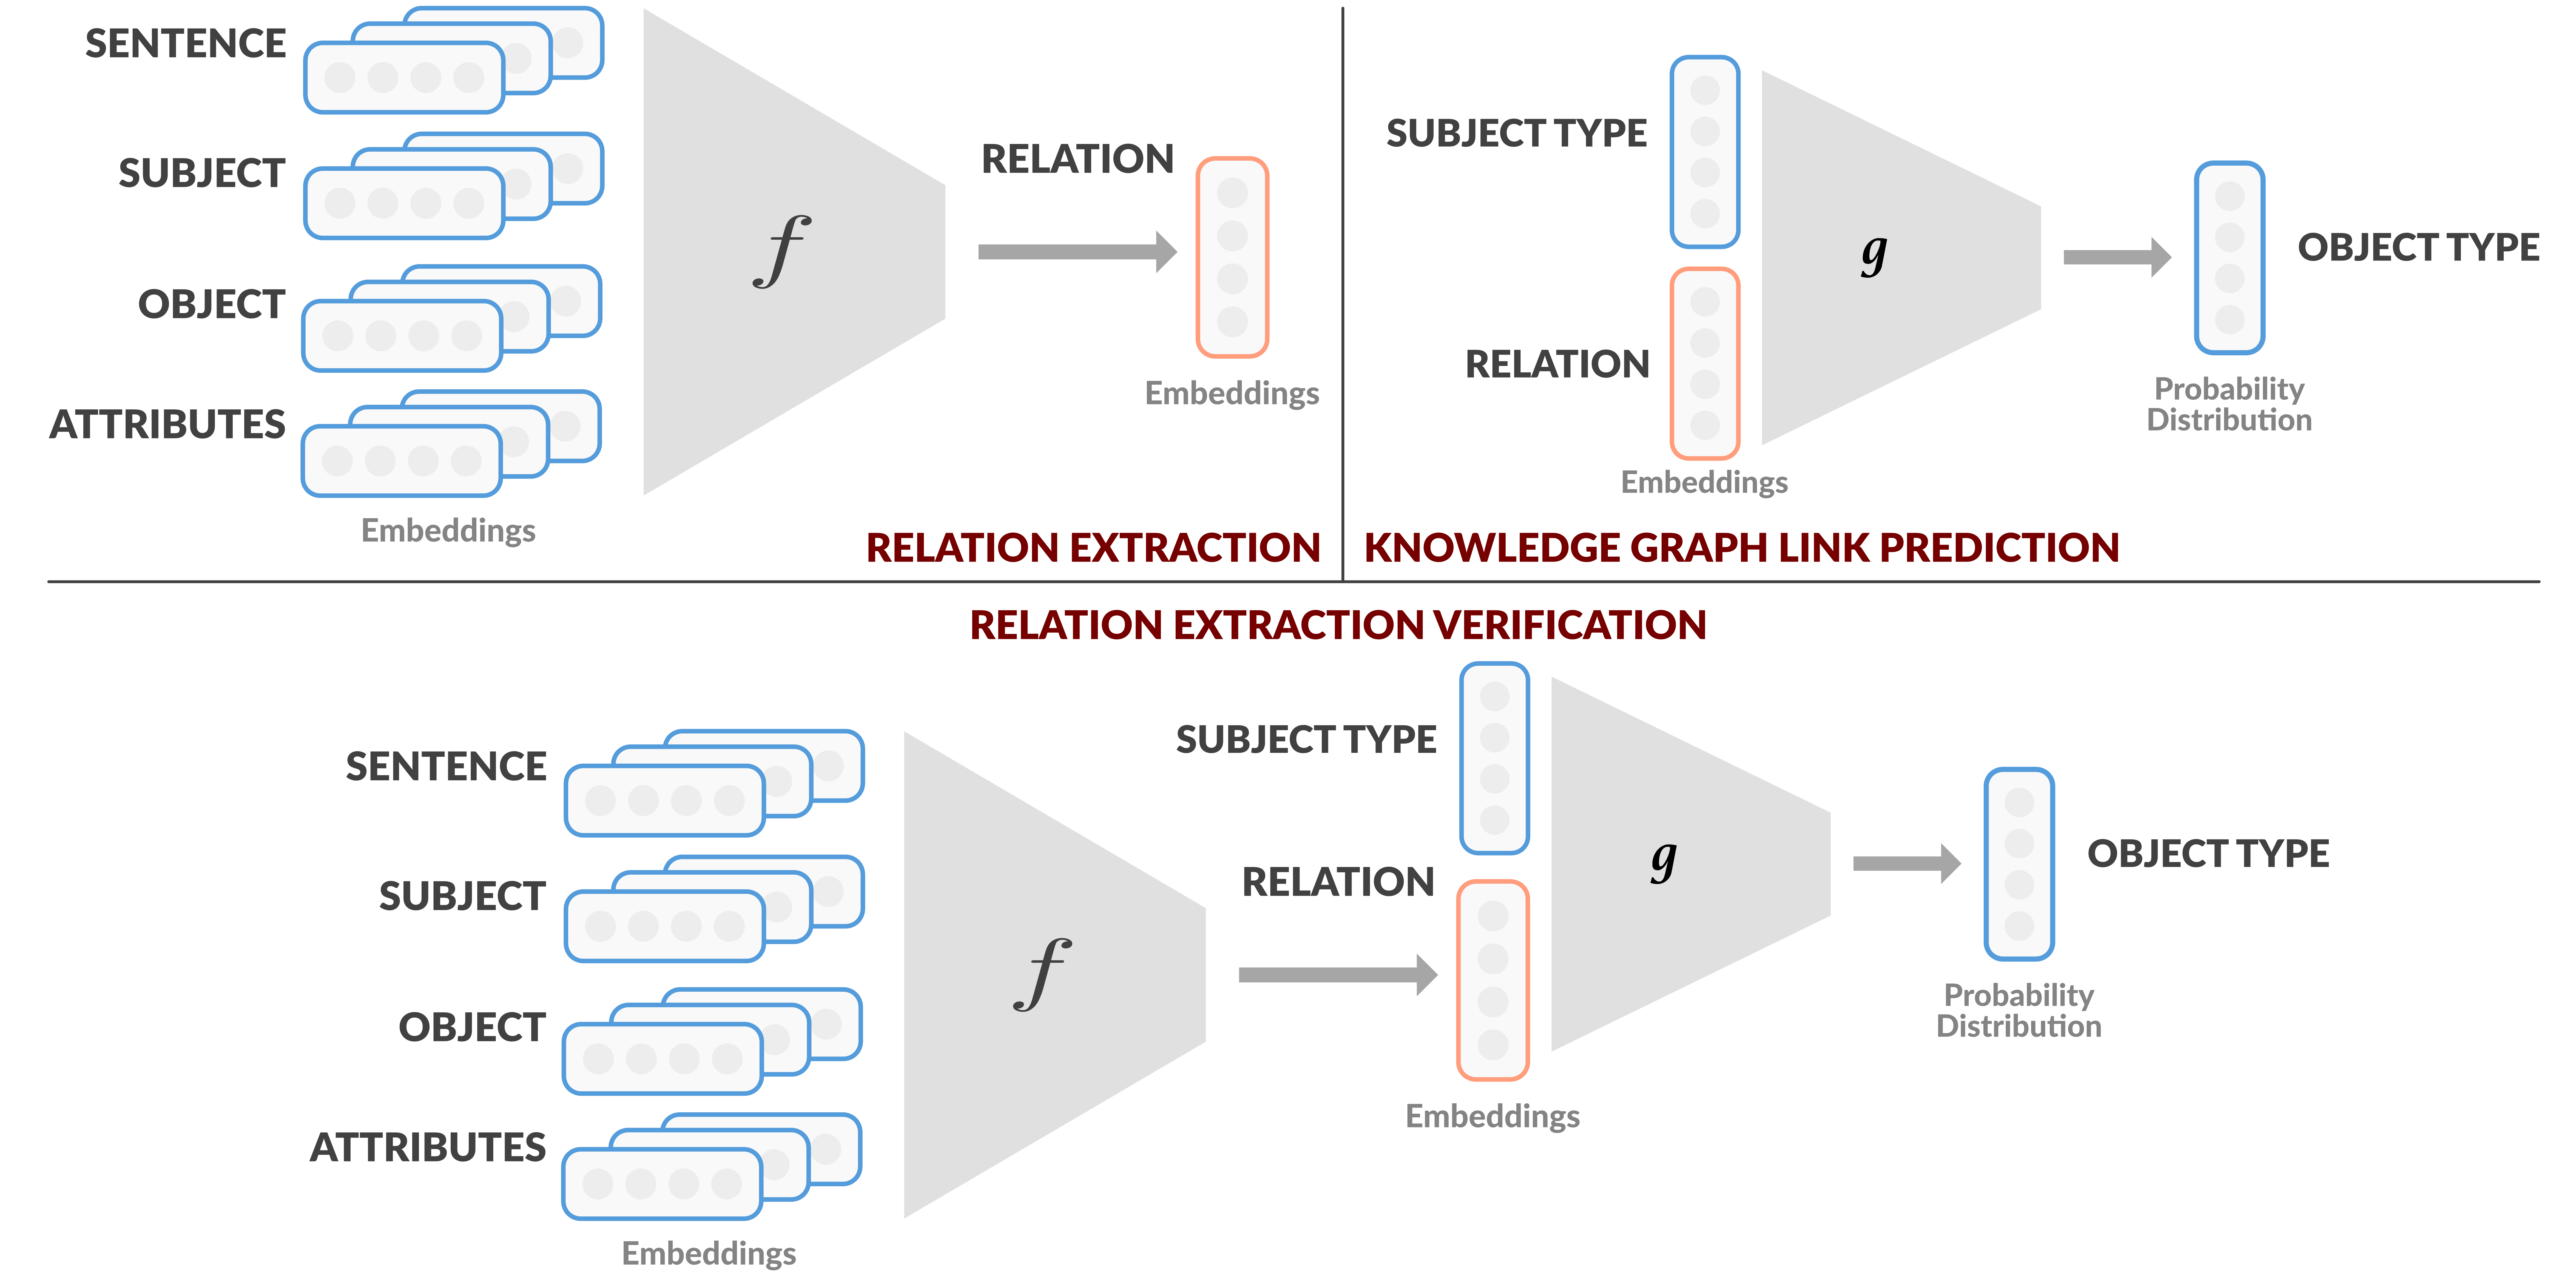
\includegraphics[width=\textwidth]{images/JRELP_figure.png}
    \caption{
        % \eapcomment{TODO: I'm hoping I'll get some time to make an overview figure / modify this one.}
        Overview of JRRELP.
        JRRELP is comprised of three loss terms: the RE loss, the KGLP loss, and the coupling loss.
        The RE loss is illustrated in the top-left quadrant, the KGLP loss is described by the top-right quadrant, and the bottom half shows the coupling loss.
        % The first task, relation extraction, is illustrated in the top-left quadrant. There, a RE model infers a relation between a sentence subject and object, given the two components, and additional sentence attributes and sentence. The second task of knowledge graph link prediction is visualized in the top-right quadrant. Given a relation and subject type -- obtained via subject {\em type-substitution}, the objective is to predict the a set of object types. Lastly, the bottom half exhibit the third task of RE verification. Similar to the second task, an RE model's relation prediction is utilized in place of the pre-existing relation to infer the set of object types.
        }
    \label{fig:JRRELP-overview}
    % \vspace{-4ex}
\end{figure*}

% Moreover, these approaches are also limited to specific KGLP model classes.

% Moreover and perhaps most importantly, these methods are not generalizable to arbitrary KGLP models as they are often designed around a specific class of KGLP models, nor do they necessarily support a broad .

% In an ideal setting, we would expect any RE model to be able to benefit from a strong KGLP model.
We propose a general framework which ties the RE and KGLP tasks cohesively into a single learning problem.
Our architecture, termed \textbf{JRRELP}---\textbf{J}ointly \textbf{R}easoning over \textbf{R}elation \textbf{E}xtraction with \textbf{L}ink \textbf{P}rediction---has the following desirable properties:
\begin{itemize}[noitemsep,topsep=0pt,label=--,leftmargin=2em]
  \item \textbf{Generality:}
    Our method can be applied to arbitrary RE and KGLP models to boost RE performance.
    % Our method can be applied to arbitrary RE and KGLP models to boost their performance.
    The only assumption JRRELP makes is that both models are trained by minimizing a loss function (which is common across all successful RE and KGLP methods).
  \item \textbf{Effective Information-Sharing:}
    JRRELP introduces a {\em cyclical} relationship between model parameters, enabling better information transfer between the learning tasks.
    Moreover, {\em all} parameters are shared across both the RE and KGLP tasks.
    % RE and KGLP task parameters, and 
    % In JRRELP, the model parameters used for RE and KGLP are {\em all} shared, enabling better information transfer between the tasks. Moreover, JRRELP establishes a novel cyclical relationship between task parameters. 
    % To the best of our knowledge, this is not true for prior work.
  \item \textbf{Performance:}
    % JRRELP boosts the performance of all baseline methods that we used in our evaluation, and achieves a new state-of-the-art. 
    JRRELP boosts the performance of all baseline methods used in our evaluation, and achieves state-of-the-art performance.
    Additionally, JRRELP-enhanced baselines even match or improve upon the performance of more expressive RE models.
    For example, we are able to train C-GCN \citep{cgcn} to match TRE \citep{tre}, even though the latter was proposed as a stronger and significantly more expressive alternative.
  \item \textbf{Efficiency:}
    JRRELP does not require any task-specific pre-training.
    It introduces a minimal overhead over the baseline methods (only $6\%$ slower per mini-batch).
    % JRRELP streamlines model training by not requiring any task-specific pretraining.
    % In JRRELP, both RE and KGLP problems are trained jointly without any task-specific pre-training, reducing training time over previous approaches \citep[e.g.,][]{han,lfds,weston-2013}.
\end{itemize}
% Additionally, JRRELP enhances the performance of weaker baselines to match that of stronger and more expressive models. For instance, applying JRRELP over C-GCN\citep{cgcn} enables it to match TRE \citep{tre}, despite the fact that TRE was proposed as a stronger and significantly more expressive alternative RE model.
% Finally, we also made an interesting observation in our experiments. 
% JRRELP on can enhance the performance of weaker baselines to match that of stronger and more expressive models.
% For example, we are able to train C-GCN \citep{cgcn} to match TRE \citep{tre}, even though the latter was proposed as a stronger and significantly more expressive alternative.
% This is explained in detail in Section~\ref{sec:experiments}.
An overview of JRRELP is shown in Figure~\ref{fig:JRRELP-overview}, and is explained in detail in Section~\ref{sec:JRRELP}.
Next, we present our proposed method and defer positioning with respect to related work until Section~\ref{sec:related_work}.
